\chapter{Generators in Peachpie}

The goal of this thesis is to enable Peachpie compiler to handle PHP generator methods while keeping as much of their original semantics as possible. That means we do not want to change their behaviour and want to enable all their features they have in PHP only now compiled to CIL and executed either by CLR or other CLI environment.
 
As noted in previous chapters\footnote{Chapter \ref{sec:3:1}} that itself is complicated because unlike the PHP runtime Zend Engine, CIL and CLR do not have a native support for generators or generally pausing the execution of a method at arbitrary points. Also, almost all other CIL based languages with generators, such as C\# or F\#, that implement them by compiler transformations have them in a substantially more limited form than PHP.

Other than that we also want to reuse existing Peachpie infrastructure and only implement generator specific bits when necessary. While this goal is not as important for our immediate work it is necessary for the project as a whole. Cluttering the compiler with logic for a feature that is not actually used as often would simply be inexcusable.

\section{Basic generators implementation}

Before dealing with all the complexities of PHP’s generators let us first explore how an implementation of their limited subset would work within Peachpie. Specifically, we will ignore \emph{yield} in exception handling blocks and expect it to be only in places where it could happen as a statement, i.e. no \emph{yield} inside an expression tree, for this chapter. 

Much like Roslyn’s approach our implementation of generators within Peachpie will also be based on transforming the original generator method into an iterator's \emph{next} method. To not to repeat ourselves we will only point out the differences in next section.

\subsection{Iterator object}

Unlike in C\# where generator methods are free to return any object implementing a \emph{IEnumerator} interface the PHP specification dictates that the returned object must be an instance of a \emph{Generator} type \citep{GenPHP, GenPHPRFC}. This means that in Peachpie we cannot just synthesize a new type for each generator method as Roslyn does it.

If we did that all reflection methods and type checks would report the actual synthesized type on the returned iterator instance instead of the \emph{Generator} type as required by PHP’s specification . We could theoretically hard code exceptions for these synthesized types into all methods that query an instance’s type but that would go against our goal to implement as little feature specific code as possible.

Instead we must create one generator type in the Peachpie’s runtime library and use it as a basis for all generator methods to return. That approach, however, carries some limitations with it. The generator type can now include only shared code and fields. That means neither a specific \emph{next} method’s implementation nor fields for lifted local variables from said method.

Other than that the \emph{Generator} type can be practically the same as the ones synthesized by Roslyn as it is a simple implementation of the PHP's \emph{Iterator} interface. It can hold captured reference to \emph{this} instance of the original generator method, state field that is needed to know what point should the \emph{next} method continue from, and fields for \emph{current} element and, since we are in PHP now, its \emph{key}. These are set before returning from the \emph{next} method and used as backing fields for the \emph{current} and \emph{key} methods on the generator.


\subsection{Next method implementation and local variables}

\subsection{Accessibility of fields on the Generator type}

\subsection{Context handling}

\begin{figure}[h]
	\centering	
	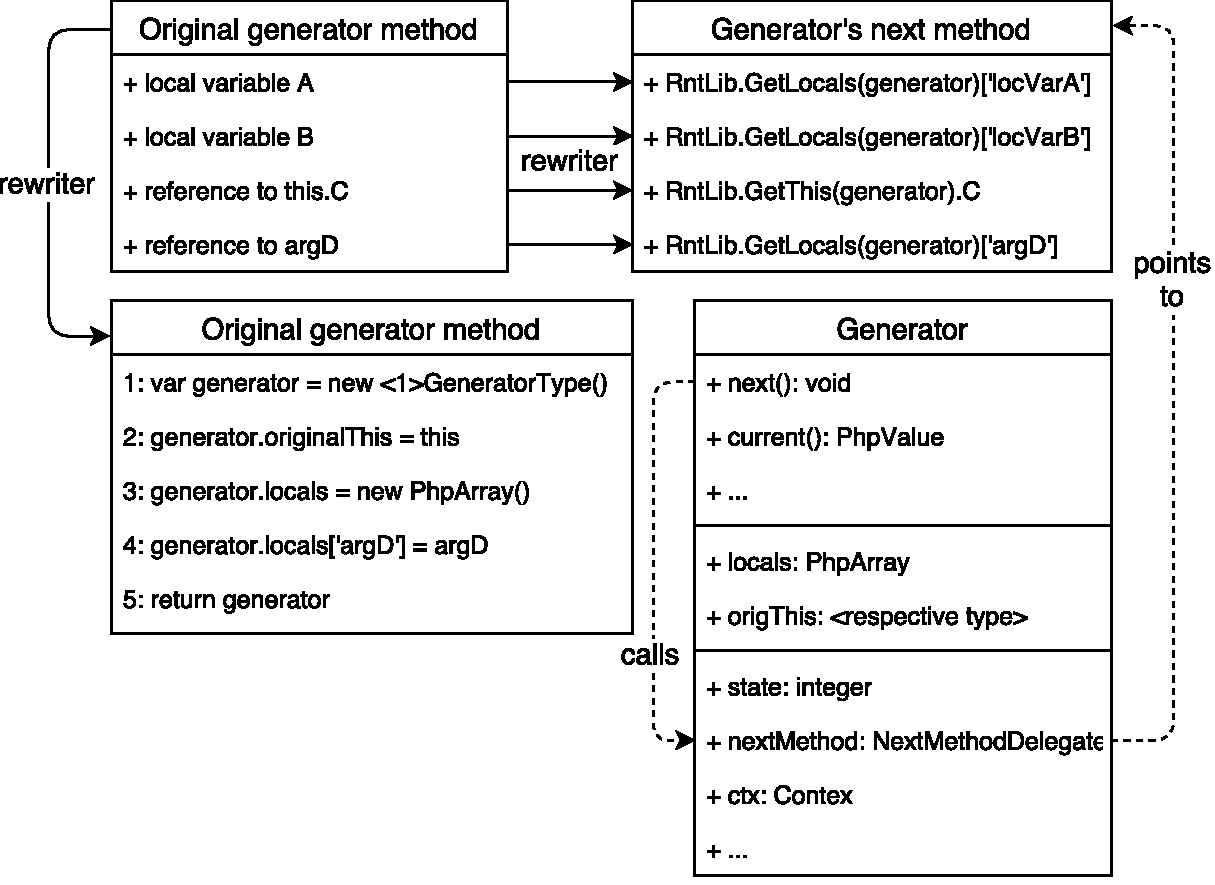
\includegraphics[scale=0.70]{../img/5_1_Generator}	
	\caption{Transformation of the generator method.}
	\label{fig5.1:Generator}
\end{figure}

\begin{listing}[H]
\caption{Simplified version of the Generator type.}
\label{list5.1:GeneratorType}
\begin{minted}{csharp}
public delegate void GeneratorStateMachineDelegate(
  Context ctx, object @this, PhpArray locals, 
  Generator gen);
public class Generator : Iterator
{
  readonly Context _ctx;
  readonly GeneratorStateMachineDelegate _stateMachineMethod;
  readonly object _this;
  readonly PhpArray _locals;
  internal int _state = 0;
  internal PhpValue _currValue, _currKey;
  public void next() =>
    _stateMachineMethod.Invoke(_ctx, _this, _locals, gen: this);
}
\end{minted}
\end{listing}


\subsection{Rewriter}

\subsection{Bound yield expression}

\begin{figure}[h]
	\centering	
	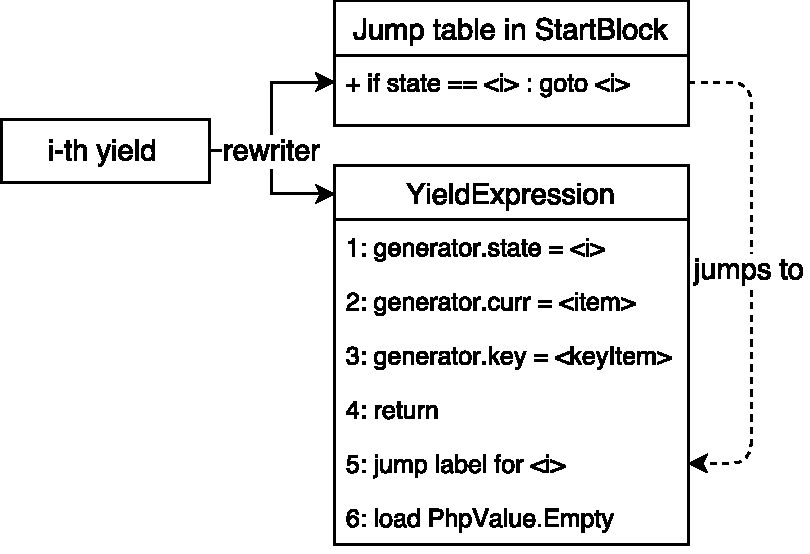
\includegraphics[scale=0.75]{../img/5_1_rewriter}	
	\caption{Rewrite of a yield expression.}
	\label{fig5.1:Rewriter}
\end{figure}


\subsection{Start block}

\subsection{Method symbol}

\section{Yield as an expression - theory}

\subsection{Possible approaches}

\subsection{Branch capture \& yield splitting}

\begin{figure}[h]
	\centering	
	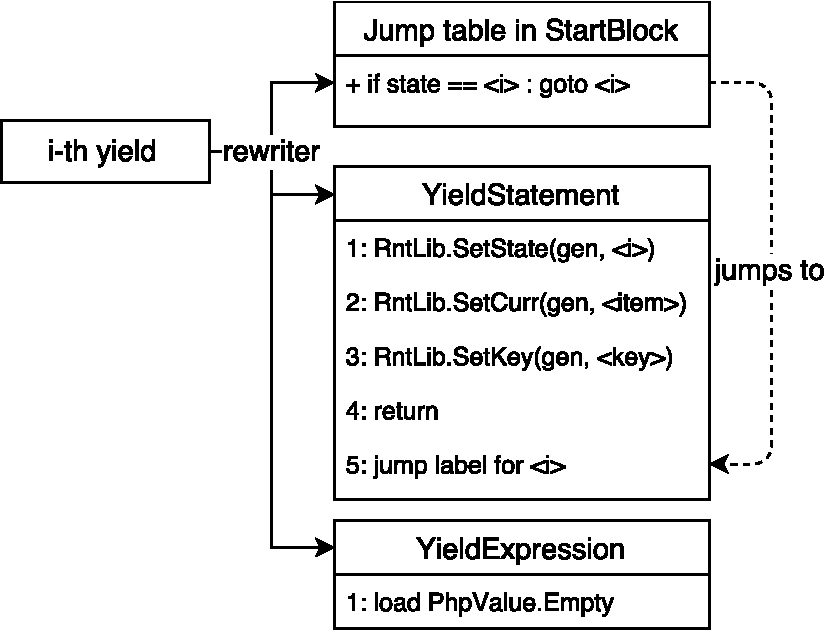
\includegraphics[scale=0.75]{../img/5_2_yieldSplitting}	
	\caption{Splitting of a yield into an expression and a statement.}
	\label{fig5.2:Splitting}
\end{figure}

\begin{figure}[h]
	\centering	
	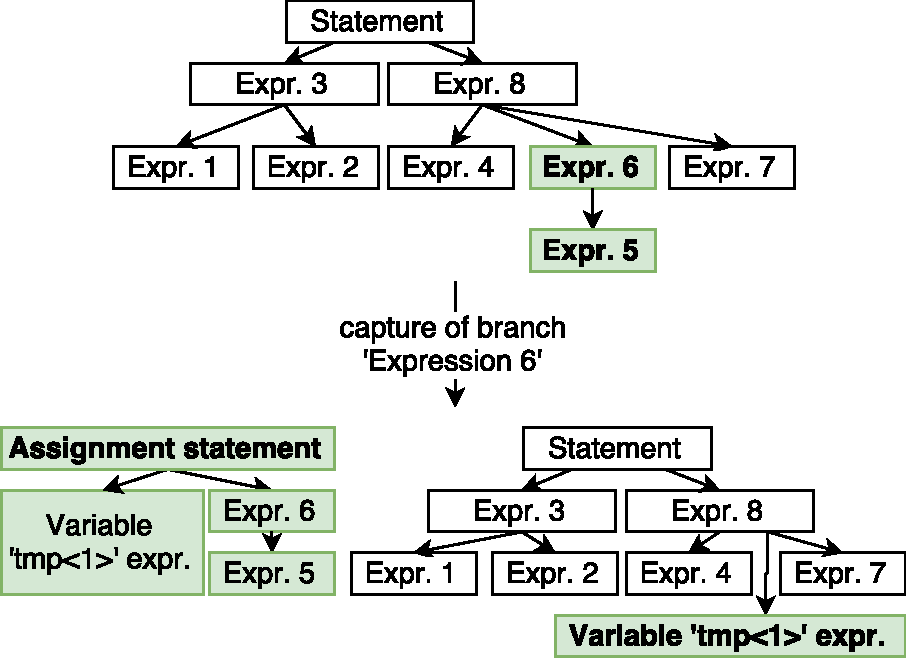
\includegraphics[scale=0.75]{../img/5_2_capturing}	
	\caption{Capturing a sole branch.}
	\label{fig5.2:CaptureBranch}
\end{figure}

\begin{figure}[h]
	\centering	
	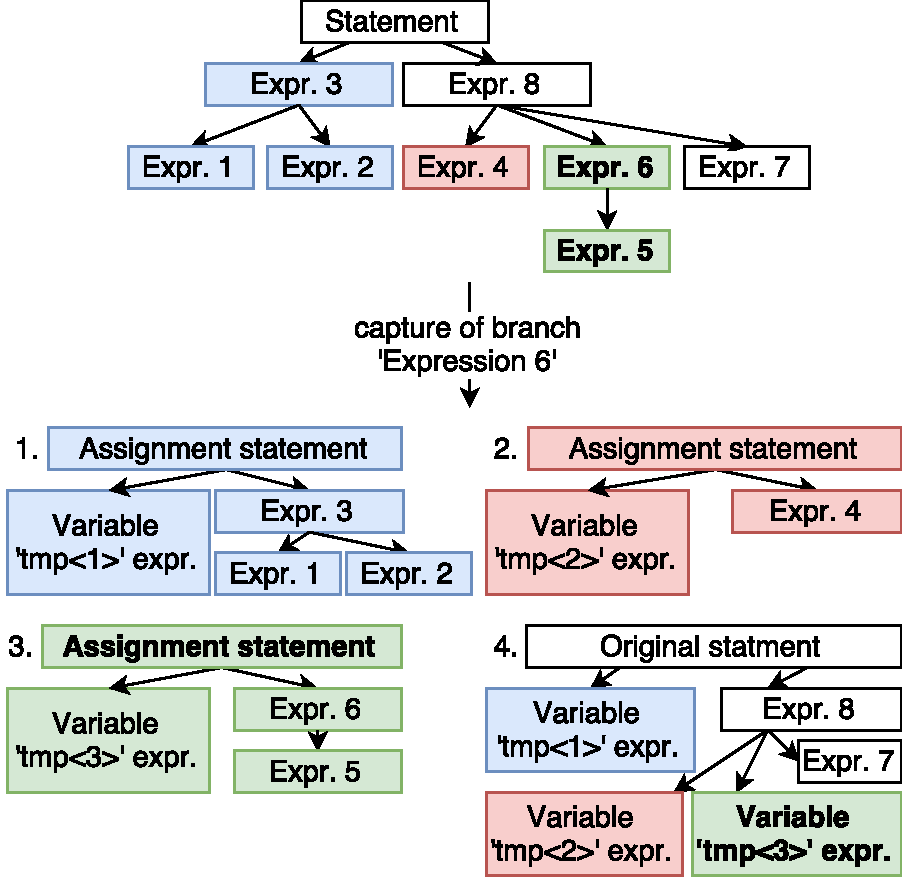
\includegraphics[scale=0.75]{../img/5_2_captureAllOnPath}	
	\caption{Capturing a whole branch while maintaining execution order.}
	\label{fig5.2:CaptureAllBranch}
\end{figure}

\subsection{Semantic tree transformation}

\begin{figure}[h]
	\centering	
	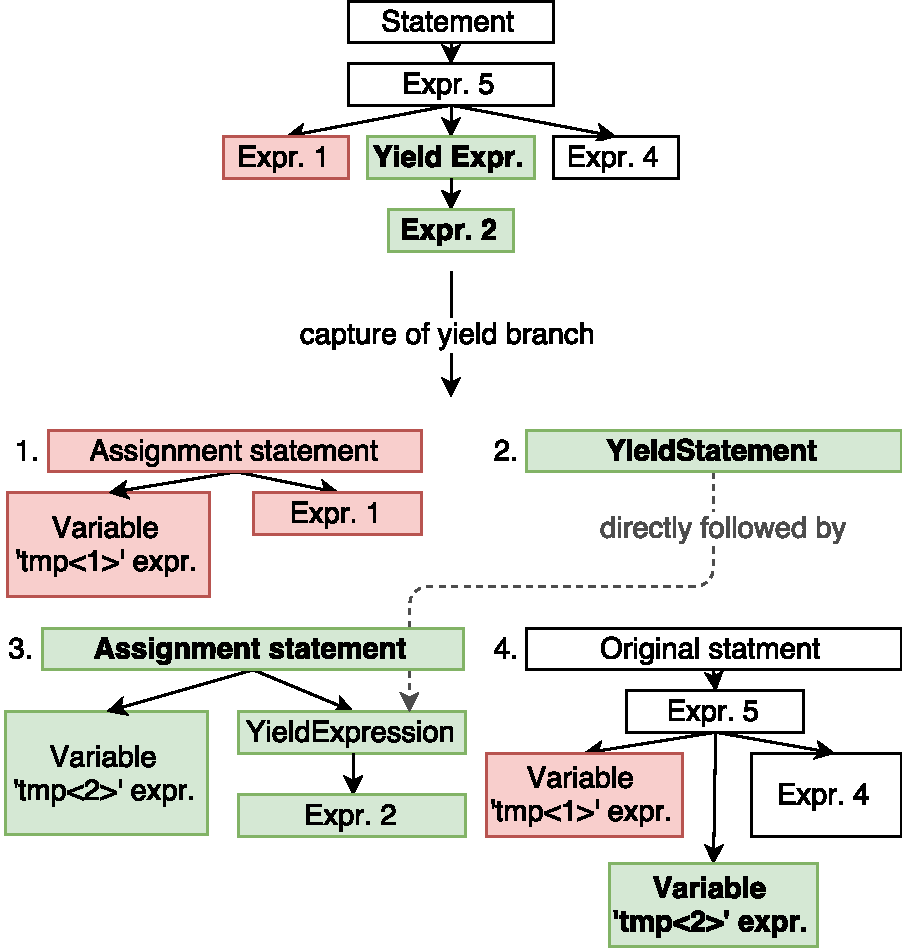
\includegraphics[scale=0.75]{../img/5_2_yieldCapturing}	
	\caption{Capturing a whole branch starting with a yield.}
	\label{fig5.2:CaptureYield}
\end{figure}

\subsection{Short circuit evaluation}

\begin{listing}[H]
\caption{Conditional expression whose captured branch is not conditioned.}
\label{list5.3:CondNotGuarded}
\begin{minted}{php}
<?php
// original expression before capturing the yield branch
$result = isTrue() ? yield 0 : “falseValue”;

$tempBranchResult = yield 0;
$result = isTrue() ? $tempBranchResult : "falseValue";
\end{minted}
\end{listing}

\begin{listing}[H]
\caption{Conditional expression whose condition is evaluated twice.}
\label{list5.3:CondTwice}
\begin{minted}{php}
<?php
if (isTrue()) { $tempBranchResult = yield 0; }
$result = isTrue() ? $tempBranchResult : "falseValue";
\end{minted}
\end{listing}

\begin{listing}[H]
\caption{Conditional expression captured correctly.}
\label{list5.3:CondCorrect}
\begin{minted}{php}
<?php
$tmpResult = isTrue();
if ($tmpResult) { $tempBranchResult = yield 0; }
$result = $tmpResult ? $tempBranchResult : "falseValue";
\end{minted}
\end{listing}

\section{Yield as an expression - implementation}

\subsection{Binding multiple elements}

\begin{figure}[h]
	\centering	
	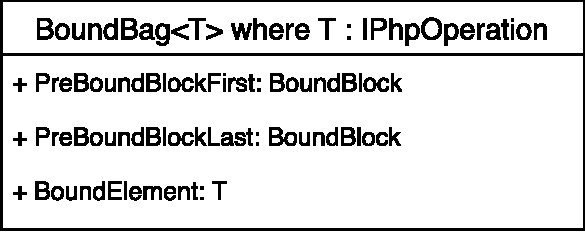
\includegraphics[scale=0.75]{../img/5_3_BoundBag}	
	\caption{Bound bag.}
	\label{fig5.3:BoundBag}
\end{figure}

\begin{figure}[h]
	\centering	
	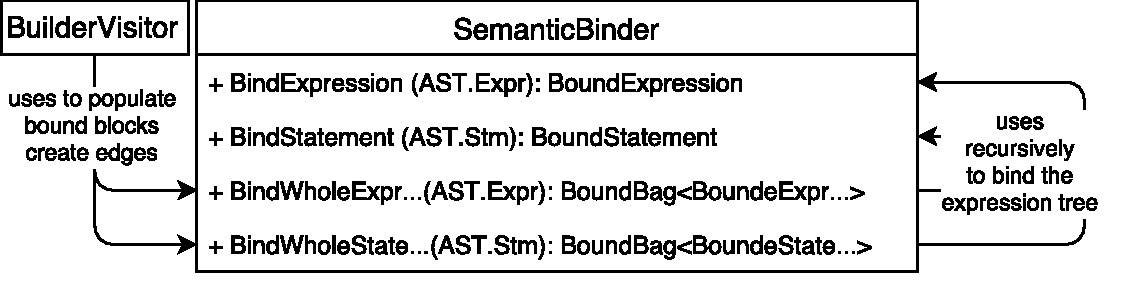
\includegraphics[scale=0.75]{../img/5_3_BoundWholeExpression}	
	\caption{Builder visitor's and semantic binder's relationship.}
	\label{fig5.3:BindWholeExpr}
\end{figure}

\begin{figure}[h]
	\centering	
	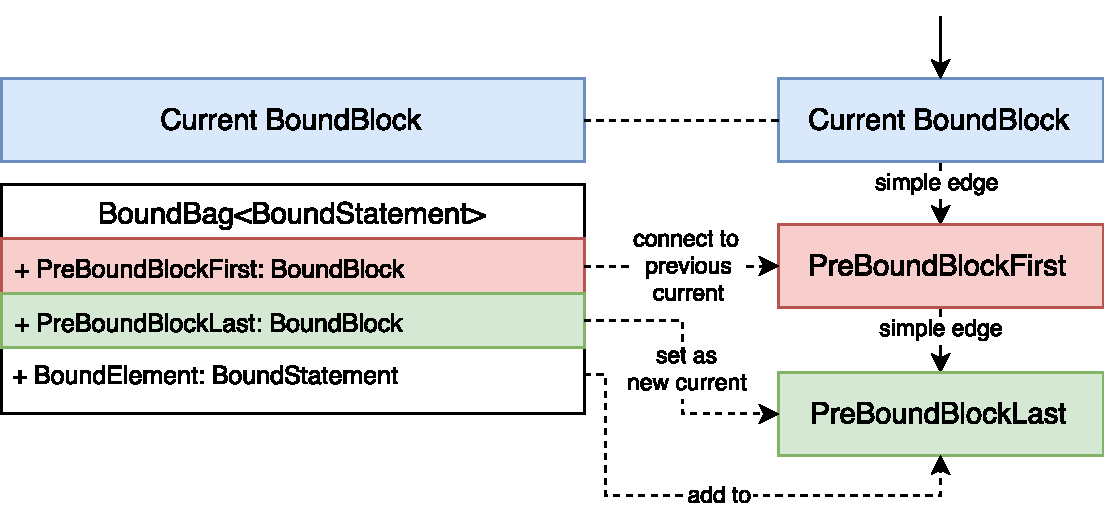
\includegraphics[scale=0.75]{../img/5_3_newStatement}	
	\caption{Connecting a bound bag as a new statement.}
	\label{fig5.3:BindNewStm}
\end{figure}

\begin{figure}[h]
	\centering	
	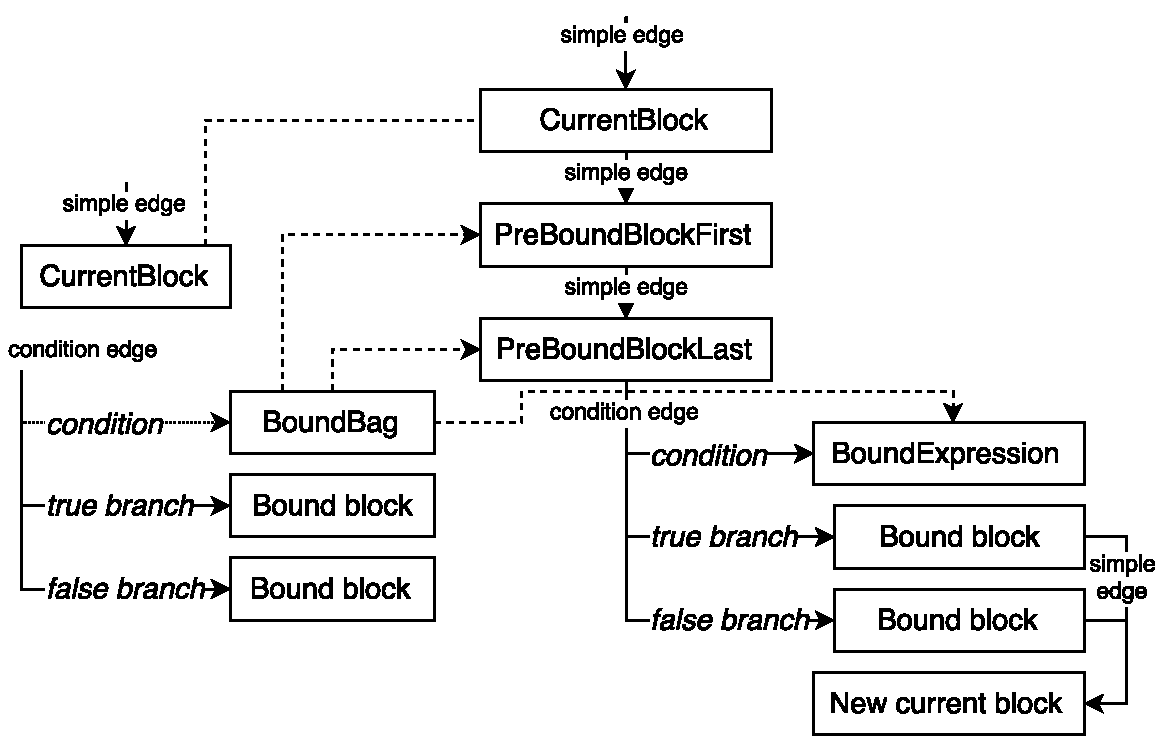
\includegraphics[scale=0.70]{../img/5_3_newInIfEdge}	
	\caption{Connecting a bound bag as a condition edge's condition.}
	\label{fig5.3:BindIfEdge}
\end{figure}

\begin{figure}[h]
	\centering	
	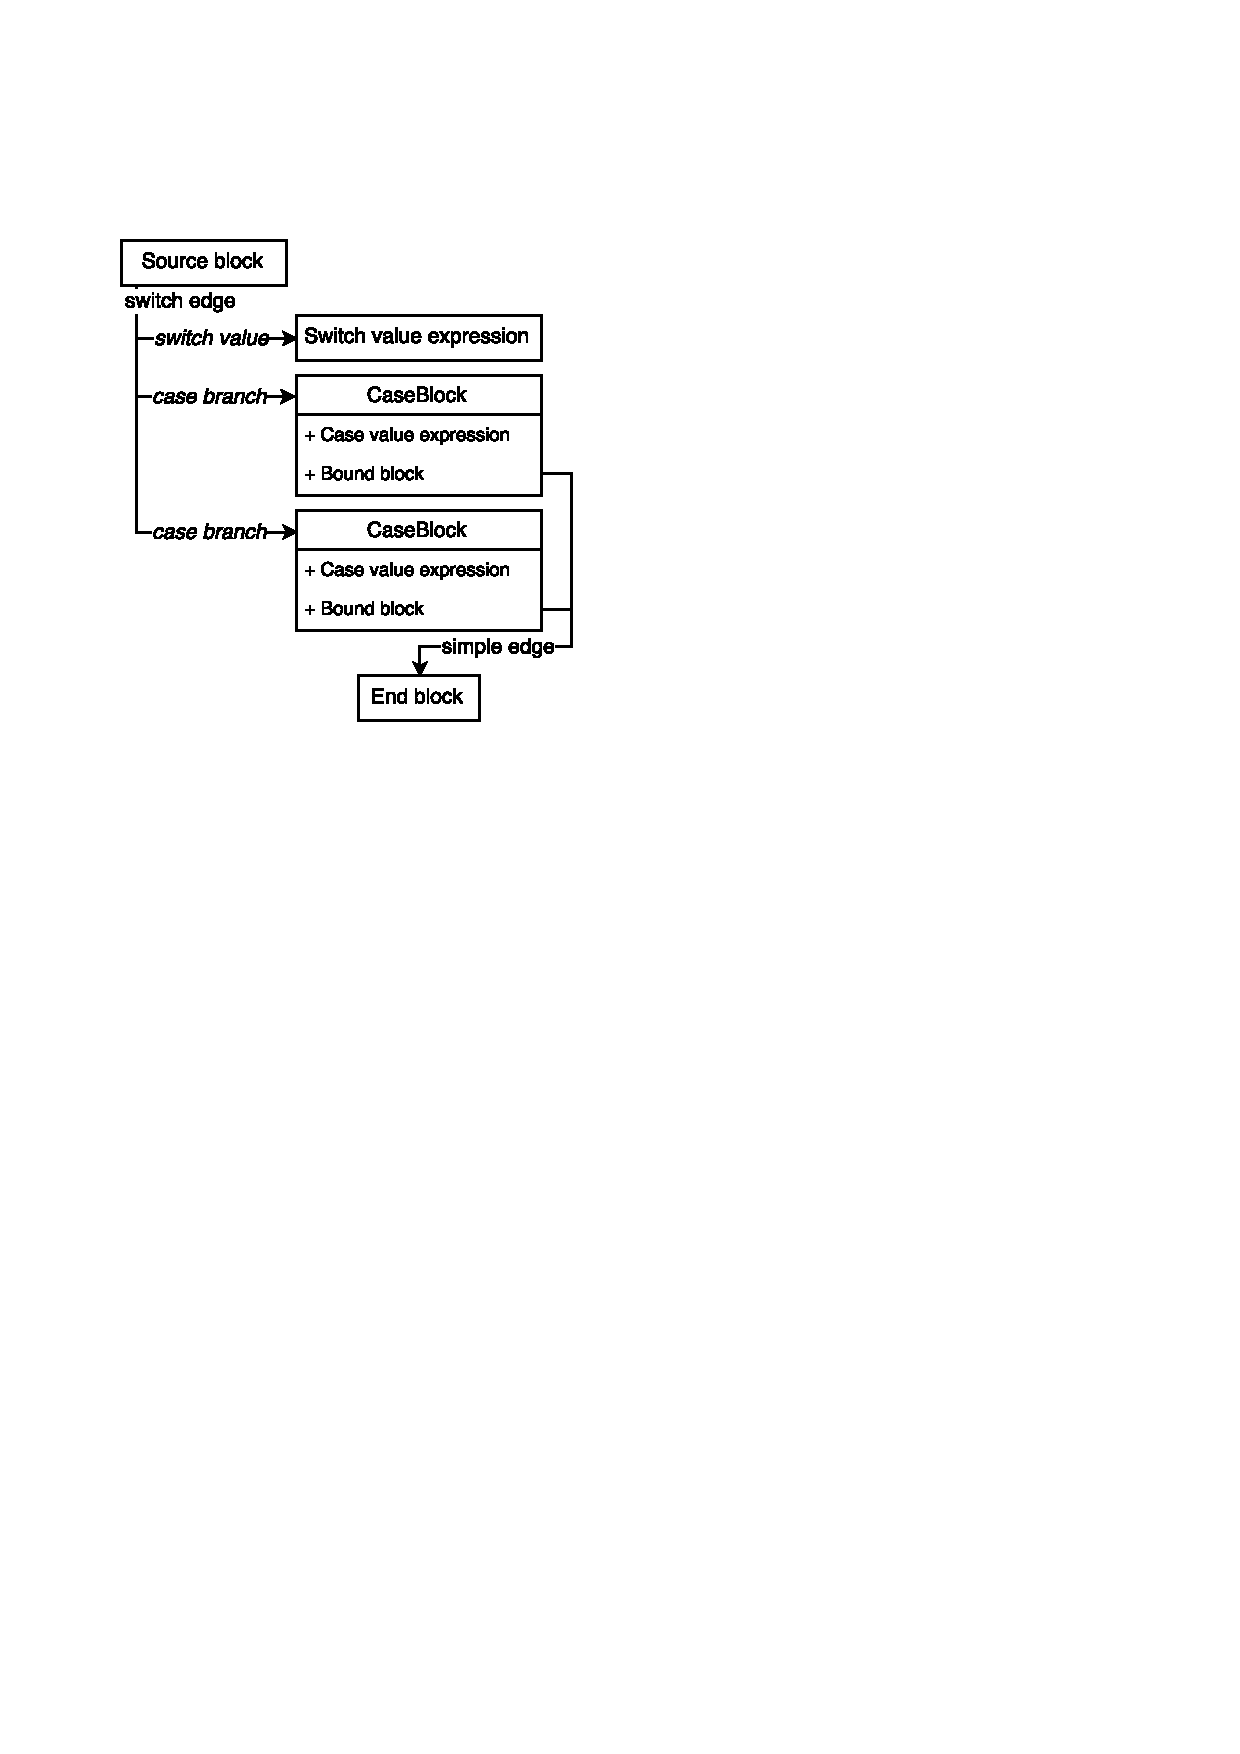
\includegraphics[scale=0.75]{../img/5_3_switchEdge}	
	\caption{Switch edge diagram.}
	\label{fig5.3:SwitchEdge}
\end{figure}

\subsection{Capturing branches with yields}

\begin{figure}[h]
	\centering	
	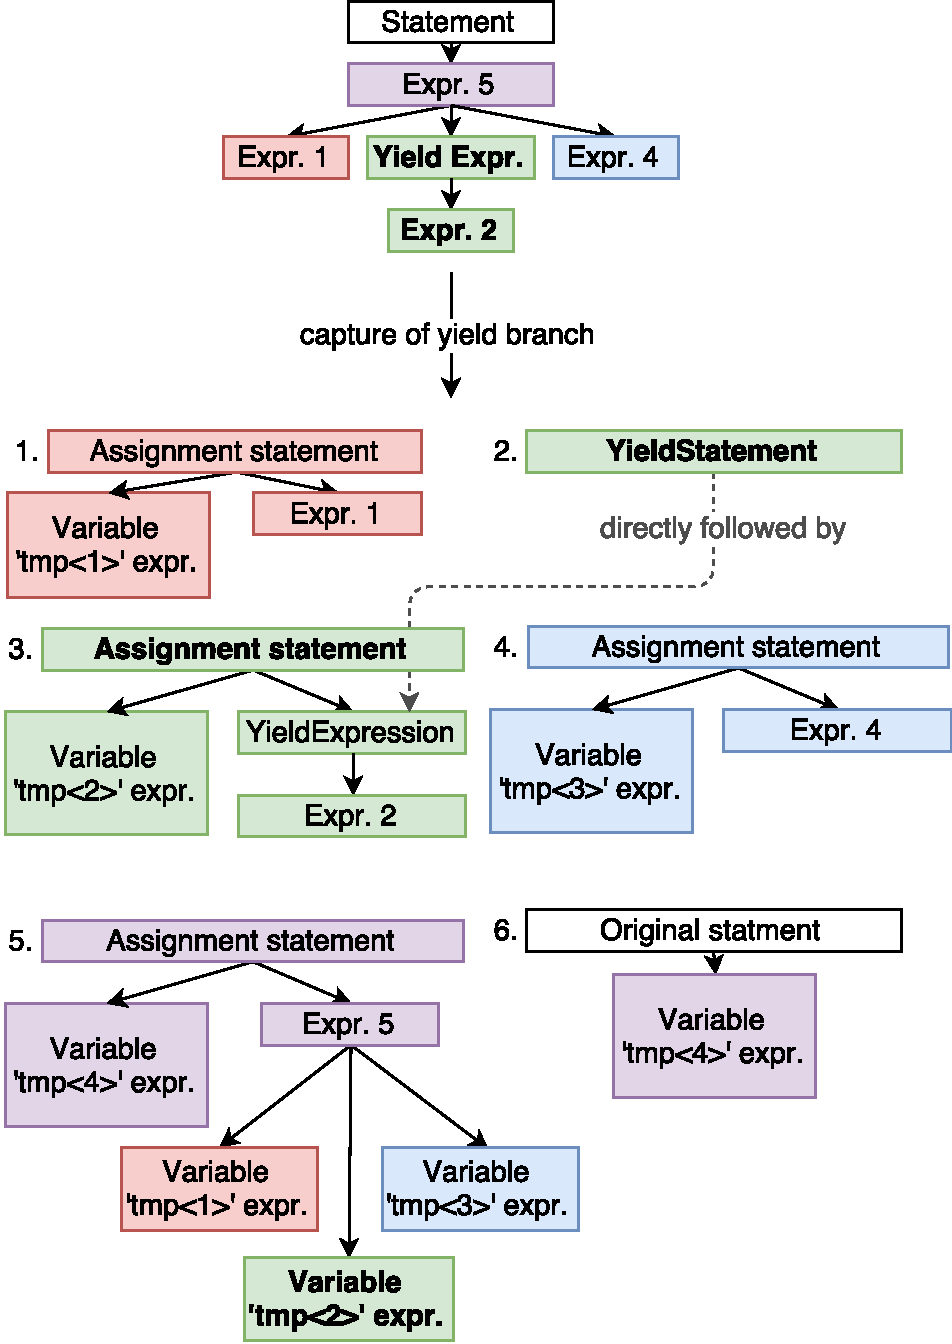
\includegraphics[scale=0.75]{../img/5_3_branchesWithYields}	
	\caption{Capturing a branch with a yield.}
	\label{fig5.3:CaptureWithYield}
\end{figure}

\subsection{Correctness of modified capturing algorithm}

\subsection{Creating and keeping the pre-bound graph}

\begin{figure}[h]
	\centering	
	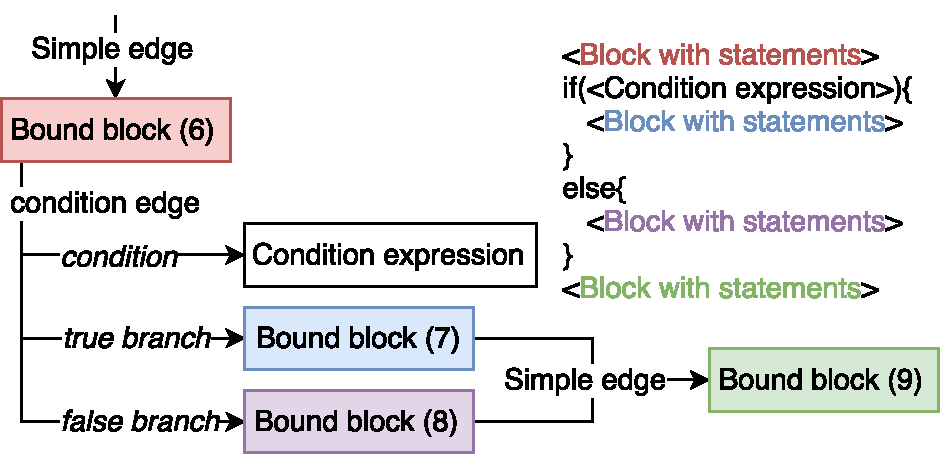
\includegraphics[scale=0.75]{../img/5_3_blockOrdinal}	
	\caption{Ordinal number of bound blocks.}
	\label{fig5.3:BlocksOrdinal}
\end{figure}

\subsection{Path between the root and yields}

\begin{figure}[h]
	\centering	
	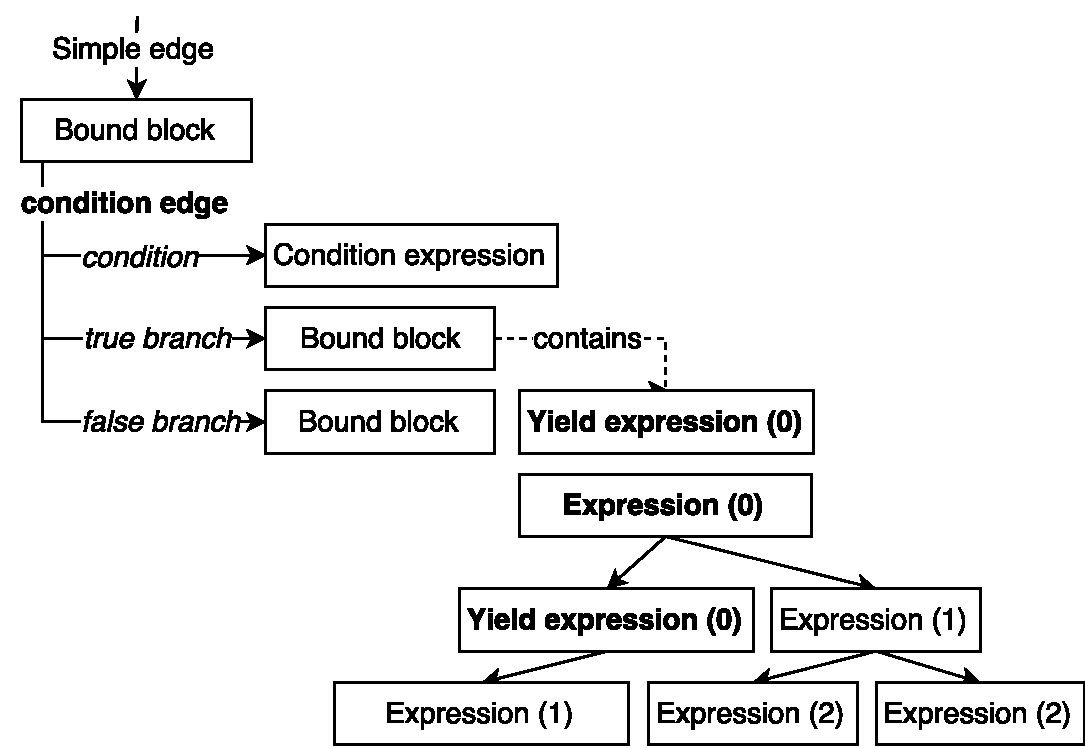
\includegraphics[scale=0.75]{../img/5_3_path}	
	\caption{Path between a yield and expression tree's root.}
	\label{fig5.3:Path}
\end{figure}

\subsection{Conditioned branches}

\begin{figure}[h]
	\centering	
	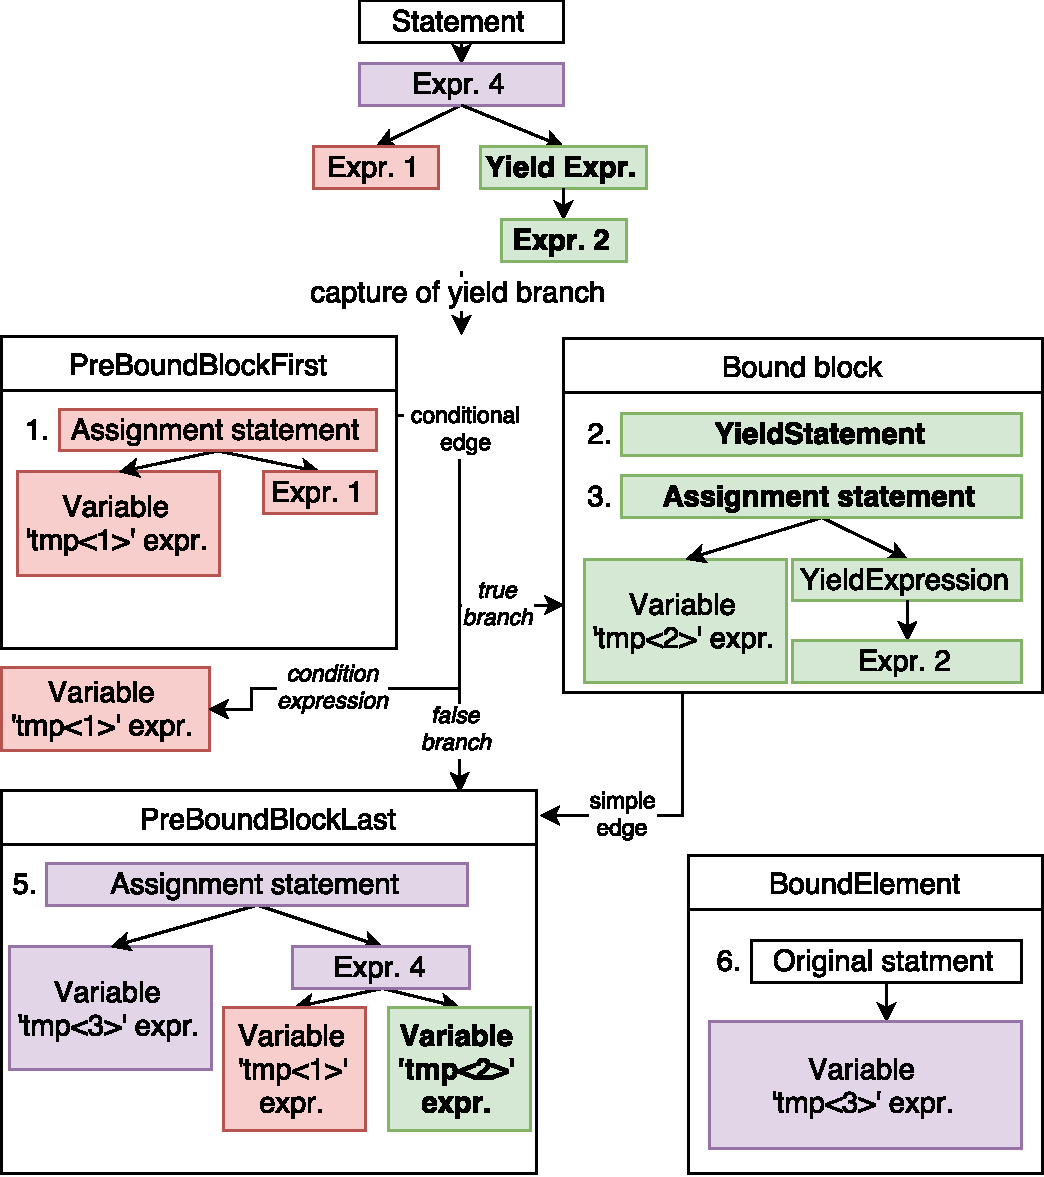
\includegraphics[scale=0.75]{../img/5_3_yieldInCond}	
	\caption{Capturing a yield in a conditioned branch.}
	\label{fig5.3:YieldInCond}
\end{figure}

\subsection{Implementation remarks}

\section{Yield in exception handling blocks}

\subsection{Yields and exception handling blocks in PHP}

\subsection{Solution in Peachpie}

\section{Future work}

\begin{figure}[h]
	\centering	
	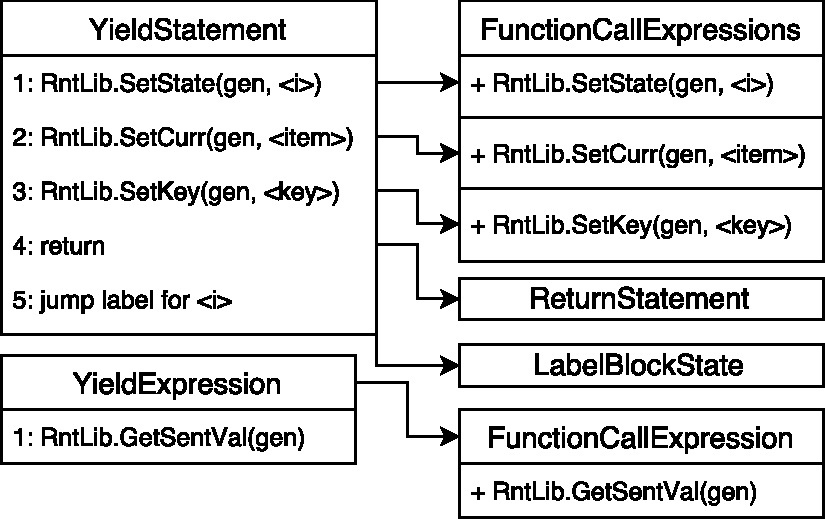
\includegraphics[scale=0.75]{../img/6_6_yieldLowering}	
	\caption{Possible lowering solution to a yield expression and a yield statement.}
	\label{fig5.5:YieldInCond}
\end{figure}

